% \protected\def\plusminus{\ensuremath{\pm}}
% \DeclareUnicodeCharacter{C2B1}{\plusminu\}newcommand{\plusminus}{\ensuremath{\pm}}

\lstset{
  inputencoding=utf8,
  literate={±}{\plusminus}1
}

\lstdefinestyle{bwC++}{
  language=C++,
  morekeywords={concept,consteval,constinit,constexpr,co_await,co_return,co_yield,requires},
  basicstyle=\ttfamily,
  keywordstyle=\bfseries,
  stringstyle=\slshape,
  commentstyle=\slshape,
  morecomment=[s][\bfseries\slshape]{/**}{*/},
  tabsize=4,
  showstringspaces=false,
  breaklines=true, breakatwhitespace=true,
  prebreak={\hbox{\quad$\rhookswarrow$}},
  postbreak={\hbox{$\lhookrightarrow$}},
  breakindent={-8pt}, breakautoindent=false,
  numbers=left, numberstyle=\tiny,
  frameshape={RYR}{N}{N}{YYY} %frame=tb,frameround=tttt
}

\lstdefinestyle{colorC++}{
  language=C++,
  morekeywords={concept,consteval,constinit,constexpr,co_await,co_return,co_yield,requires},
  basicstyle=\ttfamily,
  keywordstyle=\textcolor{blue},
  stringstyle=\slshape\textcolor{red!70!black},
  commentstyle=\slshape\textcolor{green!50!black},
  morecomment=[s][\bfseries\slshape\textcolor{green!50!black}]{/**}{*/},
  tabsize=4,
  showstringspaces=false,
  breaklines=true, breakatwhitespace=true,
  prebreak={\hbox{\quad\textcolor{red}{$\rhookswarrow$}}},
  postbreak={\hbox{\textcolor{red}{$\lhookrightarrow$}}},
  breakindent={-8pt}, breakautoindent=false,
  numbers=left, numberstyle=\tiny,
  frameshape={RYR}{N}{N}{YYY} %frame=tb,frameround=tttt
}

\lstdefinestyle{colorBash}{
  language=bash,
  basicstyle=\ttfamily,
  keywordstyle=\textcolor{blue},
  stringstyle=\slshape\textcolor{red!70!black},
  commentstyle=\slshape\textcolor{green!50!black},
  morecomment=[s][\bfseries\slshape\textcolor{green!50!black}]{/**}{*/},
  tabsize=4,
  showstringspaces=false,
  breaklines=true, breakatwhitespace=true,
  prebreak={\hbox{\quad\textcolor{red}{$\rhookswarrow$}}},
  postbreak={\hbox{\textcolor{red}{$\lhookrightarrow$}}},
  breakindent={-8pt}, breakautoindent=false,
  numbers=left, numberstyle=\tiny,
  frameshape={RYR}{N}{N}{YYY} %frame=tb,frameround=tttt
}

\lstdefinestyle{python}{
  language=Python,
  morekeywords={as},
  basicstyle=\ttfamily,
  keywordstyle=\color{blue},
  stringstyle=\color{red!70!black},
  commentstyle=\color{green!50!black},
  morecomment=[s][\bfseries\slshape\color{green!50!black}]{"""}{"""},
  tabsize=4,
  showstringspaces=false,
  breaklines=true,
  prebreak=\raisebox{0ex}[0ex][0ex]{\ensuremath{\hookleftarrow}},
  postbreak=\raisebox{0ex}[0ex][0ex]{\ensuremath{\hookrightarrow}},
  numbers=left,
  numberstyle=\tiny,
  frame=tb,
  frameround=tttt
}

The following two sections show the CMakeLists.txt files used to build the project as well as the source code itself.
I used CLion as my IDE on Windows 11 with the bundled toolchains.
Please see Figure \ref{fig:toolchains} for the toolchains setup.

\begin{figure}[H]
  \centering
  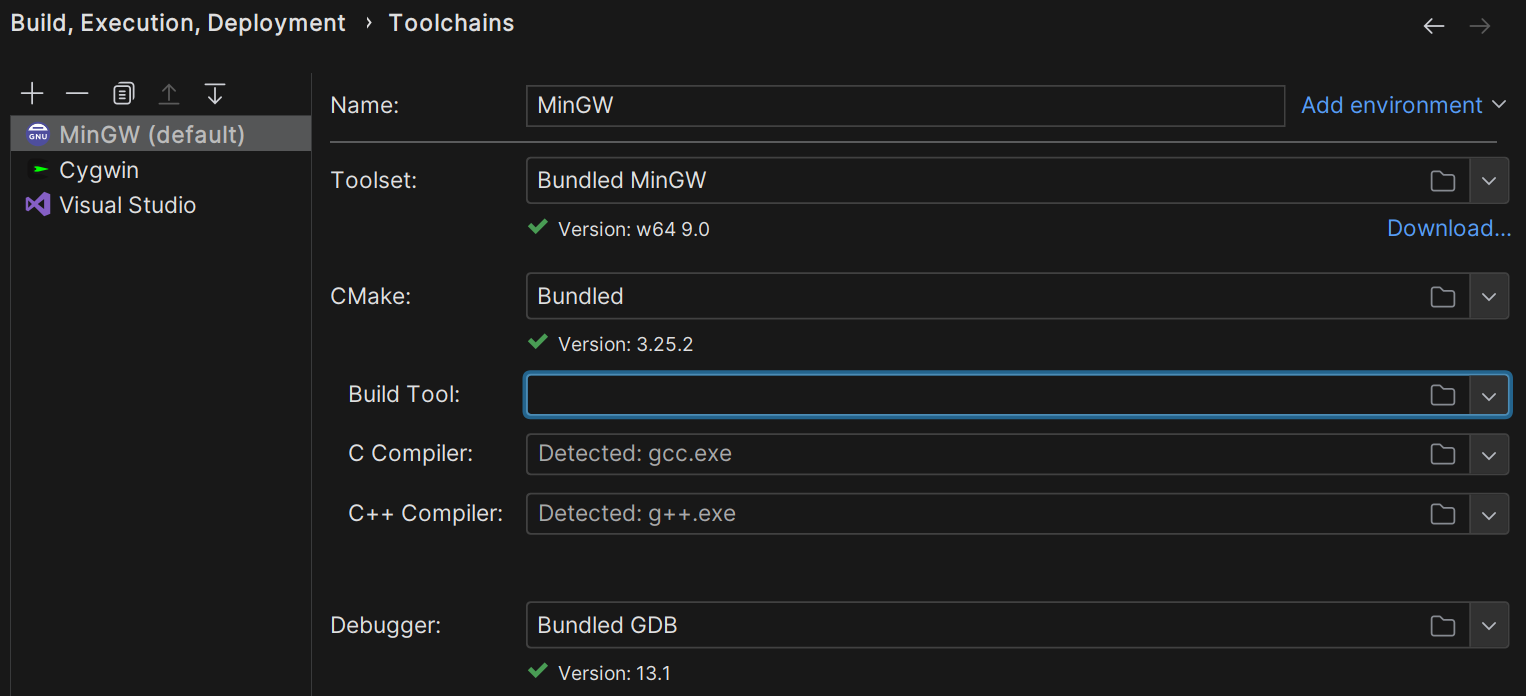
\includegraphics[width=0.8\textwidth]{toolchains.png}
  \caption{Toolchains setup in CLion.}
  \label{fig:toolchains}
\end{figure}

\begin{figure}[H]
  \centering
  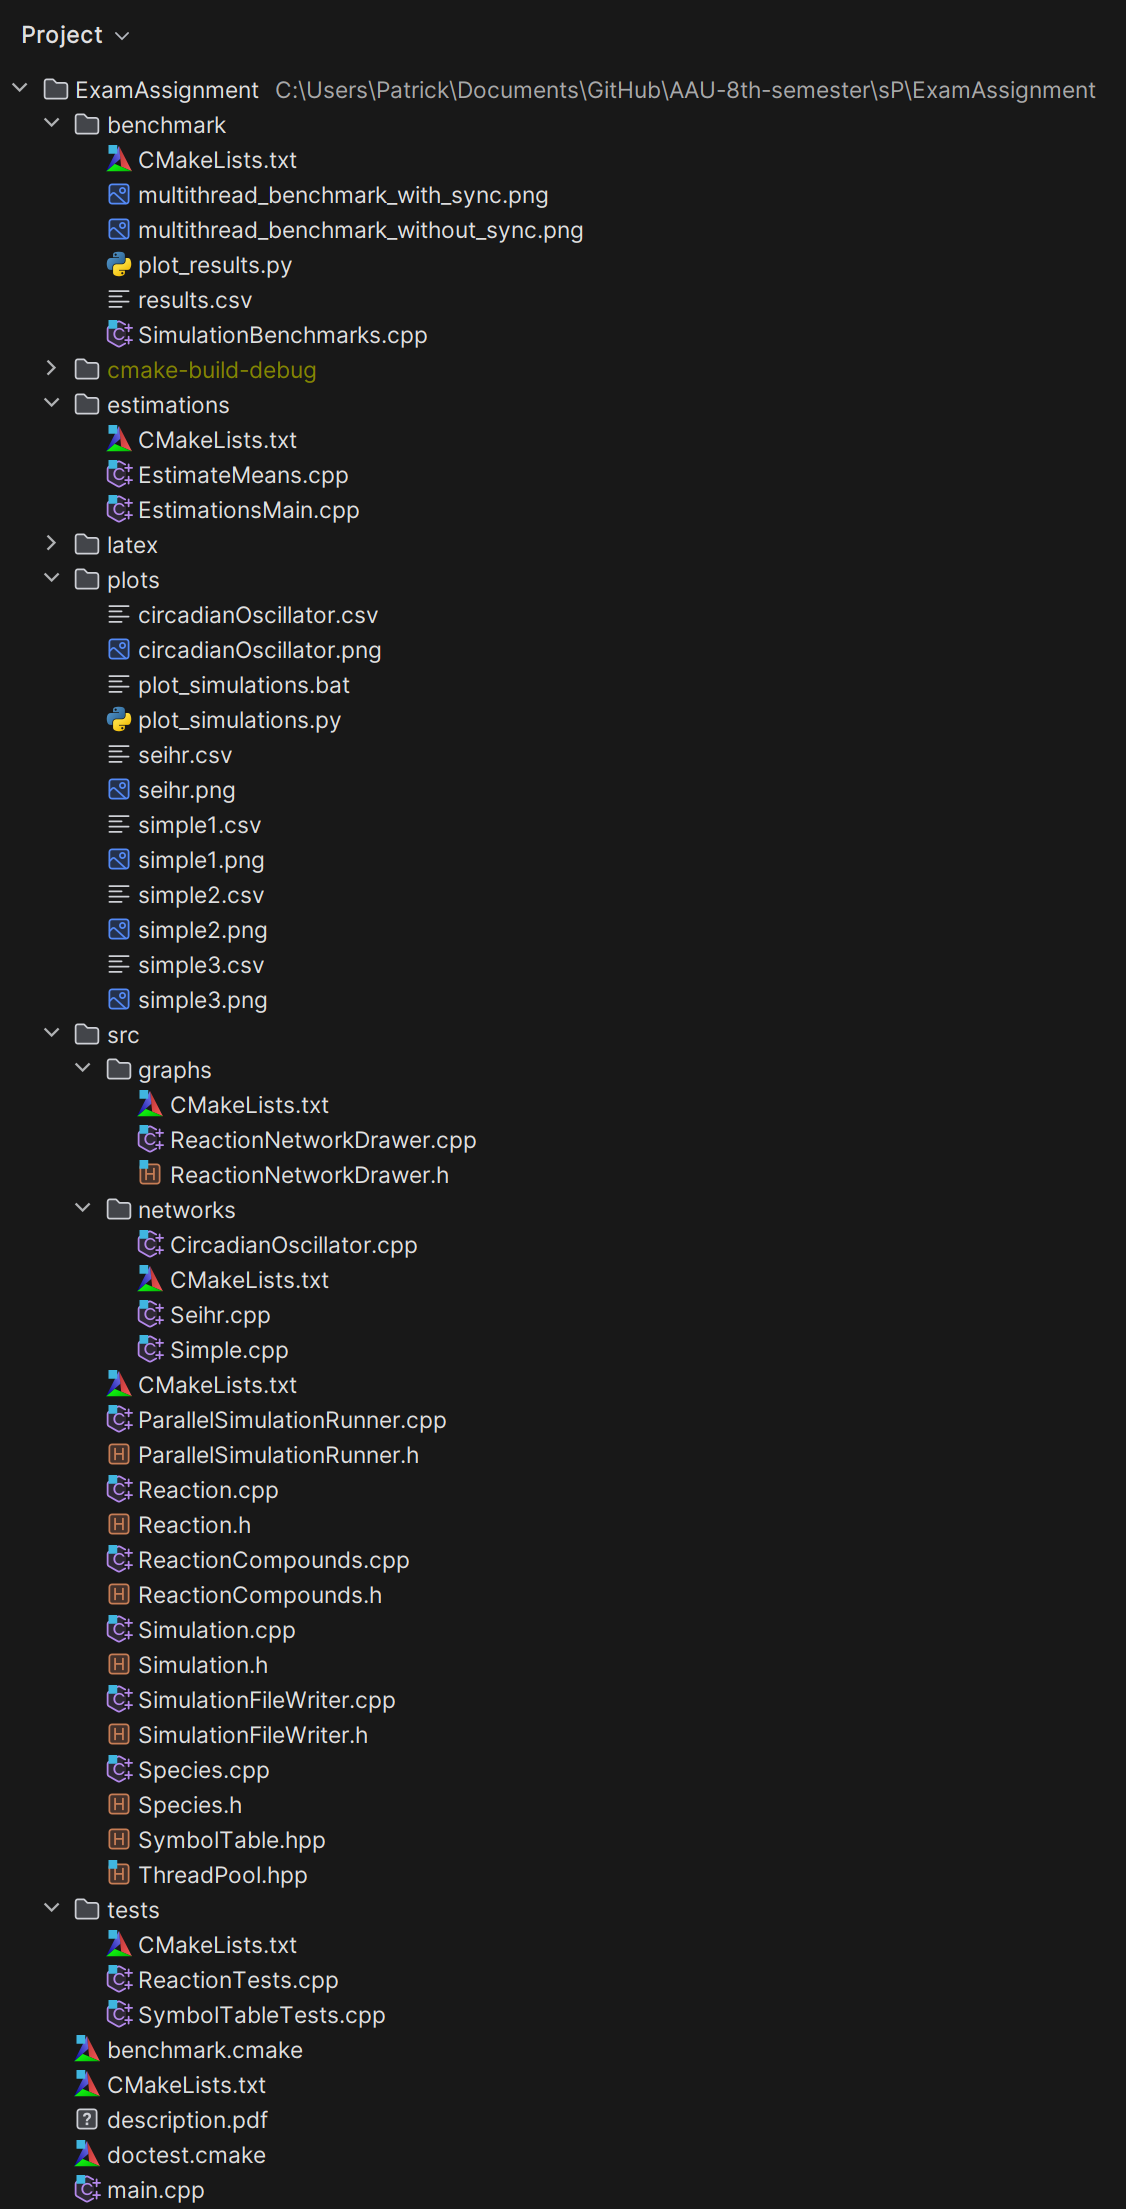
\includegraphics[width=0.675\textwidth]{project_structure.png}
  \caption{Project structure in CLion.}
  \label{fig:project_structure}
\end{figure}

In addition, Figure \ref{fig:project_structure} shows the project structure in CLion.

\subsection{CMakeLists}
The following listings show the CMakeLists.txt files used to build the project.

\lstinputlisting[style=colorBash,caption={CMakeLists.txt}]{../CMakeLists.txt}
\lstinputlisting[style=colorBash,caption={src/CMakeLists.txt}]{../src/CMakeLists.txt}
\lstinputlisting[style=colorBash,caption={src/networks/CMakeLists.txt}]{../src/networks/CMakeLists.txt}
\lstinputlisting[style=colorBash,caption={src/graphs/CMakeLists.txt}]{../src/graphs/CMakeLists.txt}
\lstinputlisting[style=colorBash,caption={estimations/CMakeLists.txt}]{../estimations/CMakeLists.txt}
\lstinputlisting[style=colorBash,caption={tests/CMakeLists.txt}]{../tests/CMakeLists.txt}
\lstinputlisting[style=colorBash,caption={benchmark/CMakeLists.txt}]{../benchmark/CMakeLists.txt}

\subsection{Source code}
The following listings show the source code for the project.
While I used the \texttt{Graphviz} C API for the graphs, I used \texttt{matplotlib} in Python for the plots, as external tools were allowed.

\lstinputlisting[style=colorC++,caption={src/Species.h}]{../src/Species.h}
\lstinputlisting[style=colorC++,caption={src/Species.cpp}]{../src/Species.cpp}

\lstinputlisting[style=colorC++,caption={src/Reaction.h}]{../src/Reaction.h}
\lstinputlisting[style=colorC++,caption={src/Reaction.cpp}]{../src/Reaction.cpp}

\lstinputlisting[style=colorC++,caption={src/ReactionCompounds.h}]{../src/ReactionCompounds.h}
\lstinputlisting[style=colorC++,caption={src/ReactionCompounds.cpp}]{../src/ReactionCompounds.cpp}

\lstinputlisting[style=colorC++,caption={src/Simulation.h}]{../src/Simulation.h}
\lstinputlisting[style=colorC++,caption={src/Simulation.cpp}]{../src/Simulation.cpp}

\lstinputlisting[style=colorC++,caption={src/ParallelSimulationRunner.h}]{../src/ParallelSimulationRunner.h}
\lstinputlisting[style=colorC++,caption={src/ParallelSimulationRunner.cpp}]{../src/ParallelSimulationRunner.cpp}

\lstinputlisting[style=colorC++,caption={src/SimulationFileWriter.h}]{../src/SimulationFileWriter.h}
\lstinputlisting[style=colorC++,caption={src/SimulationFileWriter.cpp}]{../src/SimulationFileWriter.cpp}

\lstinputlisting[style=colorC++,caption={src/SymbolTable.hpp}]{../src/SymbolTable.hpp}

\lstinputlisting[style=colorC++,caption={src/ThreadPool.hpp}]{../src/ThreadPool.hpp}

\lstinputlisting[style=colorC++,caption={src/networks/Simple.cpp}]{../src/networks/Simple.cpp}

\lstinputlisting[style=colorC++,caption={src/networks/Seihr.cpp}]{../src/networks/Seihr.cpp}

\lstinputlisting[style=colorC++,caption={src/networks/CircadianOscillator.cpp}]{../src/networks/CircadianOscillator.cpp}

\lstinputlisting[style=colorC++,caption={src/graphs/ReactionNetworkDrawer.h}]{../src/graphs/ReactionNetworkDrawer.h}
\lstinputlisting[style=colorC++,caption={src/graphs/ReactionNetworkDrawer.cpp}]{../src/graphs/ReactionNetworkDrawer.cpp}

\lstinputlisting[style=colorC++,caption={estimations/EstimateMeans.cpp}]{../estimations/EstimateMeans.cpp}
\lstinputlisting[style=colorC++,caption={EstimationsMain.cpp},label={lst:EstimationsMain.cpp}]{../estimations/EstimationsMain.cpp}

\lstinputlisting[style=colorC++,caption={tests/ReactionTests.cpp}]{../tests/ReactionTests.cpp}

\lstinputlisting[style=colorC++,caption={tests/SymbolTableTests.cpp}]{../tests/SymbolTableTests.cpp}

\lstinputlisting[style=python,caption={plots/plot\_simulations.py}]{../plots/plot_simulations.py}

\lstinputlisting[style=python,caption={benchmark/plot\_results.py}]{../benchmark/plot_results.py}

\lstinputlisting[style=colorC++,caption={benchmark/SimulationBenchmarks.cpp}]{../benchmark/SimulationBenchmarks.cpp}

\lstinputlisting[style=colorC++,caption={main.cpp}]{../main.cpp}
